\documentclass[11pt,DIV12,BCOR0mm,oneside,headings=normal,%
  numbers=noenddot,headsepline,headinclude]{scrreprt}
\usepackage[automark,headsepline]{scrpage2}
\usepackage{scrhack}                % to avoid KOMA-Script warning
\usepackage[utf8]{inputenc}         % UTF8 encoding
%\usepackage[latin1]{inputenc}      % ISO encoding
\usepackage[T1]{fontenc}
\usepackage{txfonts}                % Postscript fonts
\usepackage[ngerman,english]{babel}
\usepackage[fixlanguage]{babelbib}
\usepackage{graphicx}
\usepackage[usenames]{xcolor}
\usepackage{listings}
\usepackage[pdftex]{hyperref}       % provides \url
\usepackage{wallpaper}              % for HsH logo
\usepackage{subfigure}


% ---------------------------------------------------------

% package configuration
\KOMAoptions{headinclude}       % for scrpage2
\lstset{numbers=none,showstringspaces=false,language=Java,%
  basicstyle=\ttfamily,frame=single,rulecolor=\color{gray}}
\hypersetup{linkcolor=black,pdfborder=0 0 0}

% layout
\tolerance=2000                 % avoid overfull hboxes
\frenchspacing                  % no extra space after full stops

% ---------------------------------------------------------

\begin{document}

\selectlanguage{english}
\selectbiblanguage{english}

% title page
\thispagestyle{empty}
%\cleardoublepage
\pagenumbering{roman}

\begin{center}
  \vspace*{4\baselineskip}
  {\sffamily\bfseries\LARGE
    Redis Database Implementation\par}
  
  \vspace*{4\baselineskip}
  {\Large }

  \vfill
  {\Large }
  \begin{figure}[htb!]
  	\centerline{
\includegraphics[width=0.8\textwidth]{resources/Redis_Logo.png}}
  \end{figure}
  
  
  \vspace*{4\baselineskip}
  {\Large \par}
  
  \vspace*{4\baselineskip}
  {\Large 05.\,01.\,2017}
  
  \vspace*{4\baselineskip}
\end{center}


{\huge\textbf{Written by}} \\
\\
\\
\textbf{} \\
Florian Sander \\
florian.sander@student.hs-hannover.de \\
\\
\\
\textbf{} \\
Nicolai Böker \\
nicolai.boeker@student.hs-hannover.de \\
\\
\\
\textbf{} \\
Danar Armin \\
danaramin5889@gmail.com \\
\\
\\
\textbf{} \\
Sascha Becker \\
s.becker@wertarbyte.com \\
\\
\\
\\
\\


\tableofcontents    % Table of Contents

%\listoftables       % Tabellenverzeichnis

% main text
\newpage
\pagenumbering{arabic}
\chapter{Introduction}

The document starts with a basic introduction to Redis and is followed by a description of the scenario which is set. Afterwards a detailed plan is developed. In the end all solutions are presented with a final recommendation.

\section{The basics}
Redis is an aggregated oriented key/value store belonging to the NoSQL databases. Redis stores values with keys, where keys identify the assigned value. For extracting a specific value the key must be known. Redis keys are binary safe, which means any binary sequence can be used as a key. Also an empty string is a valid key. In Redis keys can expire. After a determined time the key is deleted automatically. Redis enables the possibility to store even complex data structures by nesting values into values or mapping objects. Redis supports the following data structures:

\begin{itemize} 
	\item Strings
	\item Lists
	\item Hashes
	\item Sets
	\item Sorted Sets
\item 	Bitmaps
	\item Message Queues
\end{itemize}

Redis provides two different storage mechanisms: Snapshotting and Append Only File Mode (AOF). A “Snapshot” holds all data in the memory. Therefore it is called “in-memory”. The data is stored onto the hard disk at a predetermined interval. These intervals can be configured by defining the number of writing operations and a time limit. Reloading the past operations to retrieve the primary state of the data after a system crash is an advantage of this method. With “AOF” every writing operations is stored onto disk immediately.

When storing strings to a Redis database the command “SET” is used. This way a value is placed to a new key. “SET” overwrites values of existing keys. So “SET” updates the value of existing keys. For retrieving the value “GET” is run. For each data type shown above exists different commands, which operates more or less the same way. Redis does not have a declarative query language. All queries in Redis are based on these commands. They can not be modified, except for the arguments, that can be passed over a command to another. The internal use of these commands is imperative. Having several single commands they can be combined to a single atomic transaction. For this Redis provides pipelining. If a command fails the whole transaction also fails. There are two transaction guarantees:
\chapter{Work Process}

Our team consists of four members. We started early with reading documentations about Redis and searched for code snippets to see how the magic is done. After we established a basic understanding we used our newly won knowledge to define a general data model which is detailed described in a later section. Based on this model we followed up different paths of implementation. Each path ended in a successful and usable solution. While working on different ways we shared our experiences, so that everyone is able to understand how things were managed. We learned from each other.

\section{Scenario}

As an example scenario, we will use network data stored in Redis and queried over various use cases. Storing and analyzing network data is important for security. By capturing the network flow we can look into two different granularities, the flow level and the packet level. In this scenario we will look at the packet level.

\subsection{Queries}
In order to analyze the network data we had been given various queries which should be implemented with redis. These are the queries we had to solve:
\begin{itemize}
	\item Query 1:
Retrieve all active connections at a certain point of time. Whereas active means that a package existed within the last second

\item Query 2:
Retrieve the overall data volume per minute for all connections between IP a.b.c.d and IP w.x.y.z

\item Query 3:
Retrieve all hosts that had connections to IP a.b.c.d on the HTTP port.

\item Query 4:
Retrieve all hosts that had incoming connections on well-known ports

\item Query 5:
Retrieve all packages that contain the byte sequence 0x35 0xAF 0xF8

\item Query 6:
Retrieve all hosts that had connections to outside hosts

\end{itemize}

\section{The Plan}

With the given scenario it was planned to have two different entities. One called “package” holding all for the queries needed attributes like “timestamp” or “source address” and the second called “data” for storing the raw data of the ethernet packages. Having two entities requires an association connecting these two objects. But first the objects must be created. Redis provides a suitable data type for doing so: Hashes. A hash consists of a several key-value fields while a prefixed key identifies a single hash. Addressing this key means getting the whole hash with all its fields. To search for specific hashes incremental numerical indexes should be generated. The same goes for each field of the hash. Additional to a field key a numerical index should be defined. This way those fields’ values of several hashes can be aggregated in a range. 

  \begin{figure}[htb!]
	\centerline{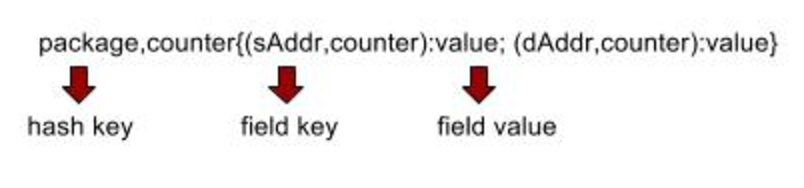
\includegraphics[width=0.8\textwidth]{resources/plan.png}}
\end{figure}

Converting the pseudo code into a valid Redis command it would look like this:

redis.hmset((‘package’,counter),{‘sAddr’,counter: sAddr})

Each field inside a single hash is an attribute of an ethernet packet. These attributes are labeled the following:
\begin{itemize}
	\item timestamp as Integer
	\item sourceAdress as Long
	\item sourceAdressPrivate as Boolean
	\item sourcePort as Integer
\item 	sourcePortWellKnown as Boolean
\item 	destinationAdress as Long
\item 	destinationAdressPrivate as Boolean
\item 	destinationPort as Integer
\item 	destinationPortWellKnown as Boolean
\end{itemize}

For the “data” entity in contrast simple Strings are applied. These strings should store the attributes “data” and “data.length”: redis.set(payload, data) and redis.set(payloadLength, data.length)
Because Redis provides commands to get any key and its value, needing an association between the “data” and “package” is left out. Instead each entity could be accessed directly. When the need to address both entities comes up, multiple commands can be combined to do so. 

All data should be stored persistent and therefore written onto disk immediately. In order to achieve this the AOF mechanism should be implemented. 

The appealed indexes are kind of pre-processing. Further pre-processing is necessary regarding to check whether a source or a destination IP is private or not. The same is valid if a port is well-known. A port is well-known when its port number is lower than 1024. And a port is a Http-port when its number is 80. Private IPs vary from 10.*.*.* over 172.[16-32].*.* to 192.168.*.*. The only planned post-processing should contain the summing of the data volume per minute. 

\chapter{Solutions}
This part of the documentation is split up into three sections due to the presence of three various solutions based on different technologies. Each section describes the methodical process of developing the final program and explains the changes from what was originally planned. All solutions are compared with each other. At last there is a recommendation which solution would fit best to the given scenario. 

\chapter{Store all, process everything later}
This solution was realized with the underlying programming language Java. The used framework for Redis is called Jedis. This solution was the first approach, the idea was to just simply store all the references for the specific paket, very similar to foreign Keys in relational Databases. On the other hand this means postprocessing with Java. The repository can be cloned at this address:
\url{ https://github.com/SirSandmann/redis_dataimport}
The structure of the data in redis for this approach looks like this:

  \begin{figure}[H]
	\centerline{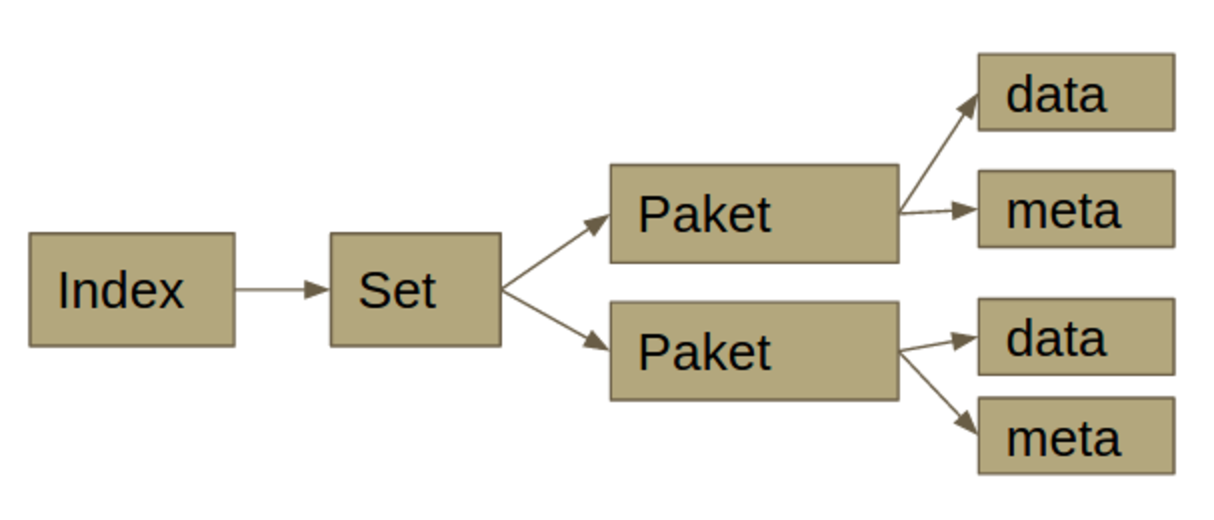
\includegraphics[width=0.8\textwidth]{resources/solution1-1.png}}
\end{figure}

All packets are seperated into the actual data and the meta data of the package, like in the original plan. The packets are in this approach two separated entities, realized with hashmaps in redis. Each packet has a unique number (e.g. 3230:meta for the meta data entity) which can be referenced. The references to the number of the packets are stores in a set. Here it gets a bit complicated. These sets are references by indexes holding the value e.g. indexSets:sourcePort:79 for the key of the set holding all the unique packet numbers. With this chaining post processing is necessary. Reviewing this solution the step with the indexes referencing a set is unnecessary, because the set could have been directly put into the index. The following screenshot shows the data structure in this approach within the Redis Desktop manager.

  \begin{figure}[H]
	\centerline{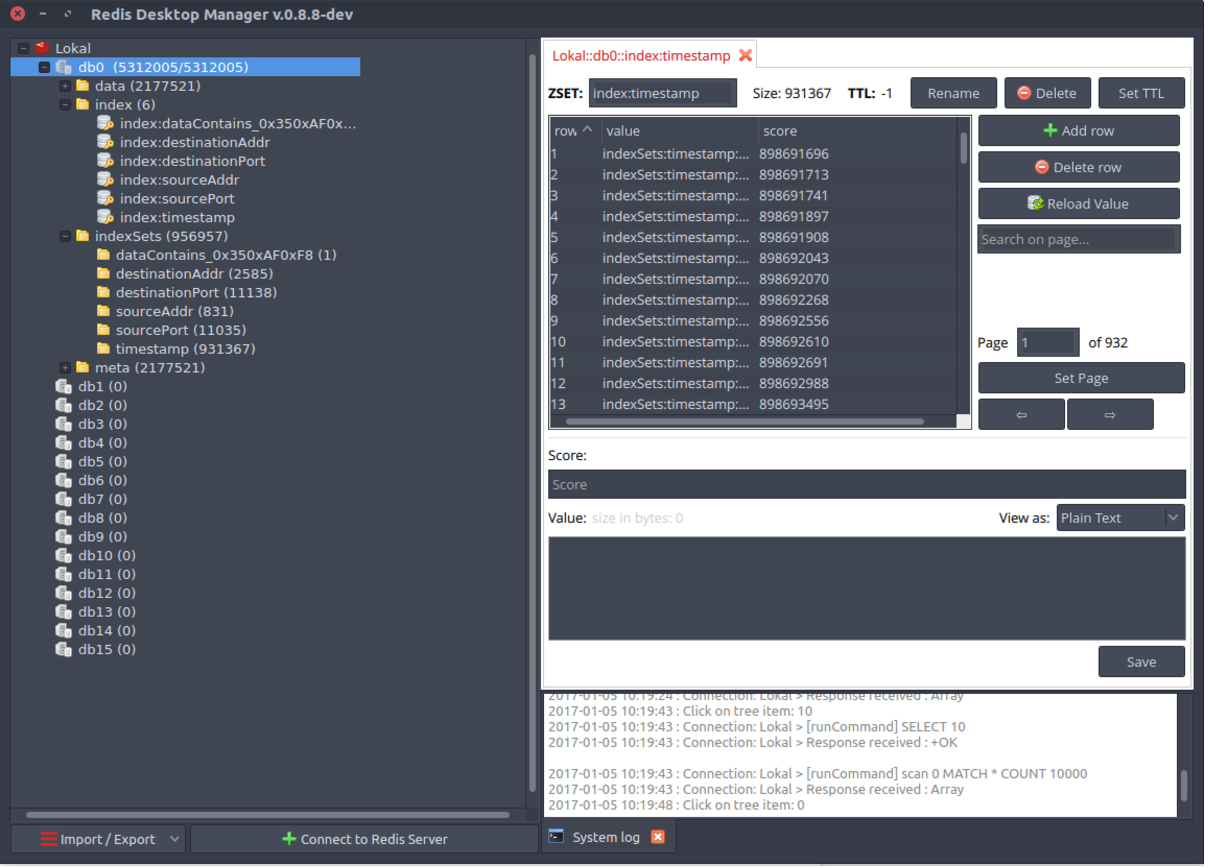
\includegraphics[width=1.0\textwidth]{resources/solution1-2.png}}
\end{figure}
The index(6) contains all characteristics of the indexed data. The indexSets(956957) contains sets of all packageIDs with the specific characteristics the Set name specifies. These sets reference the data within the meta(2177521) and the data(2177521) space.

\chapter{Store only what was asked for}
This approach follows the concept of pure application, or in this case query based database. It was implemented with nodejs as the ground framework, pcap for network sniffing, hapi for the REST api and swagger for the REST gui visualisation. You can clone this repo here: \url{https://github.com/saschb2b/redis-pcap-monitor}

The idea is to write specific data into different redis data types as the data is being sniffed. So every write operation is handled in the “on packet” callback (\ref{loop}).
  \begin{figure}[H]
	\centerline{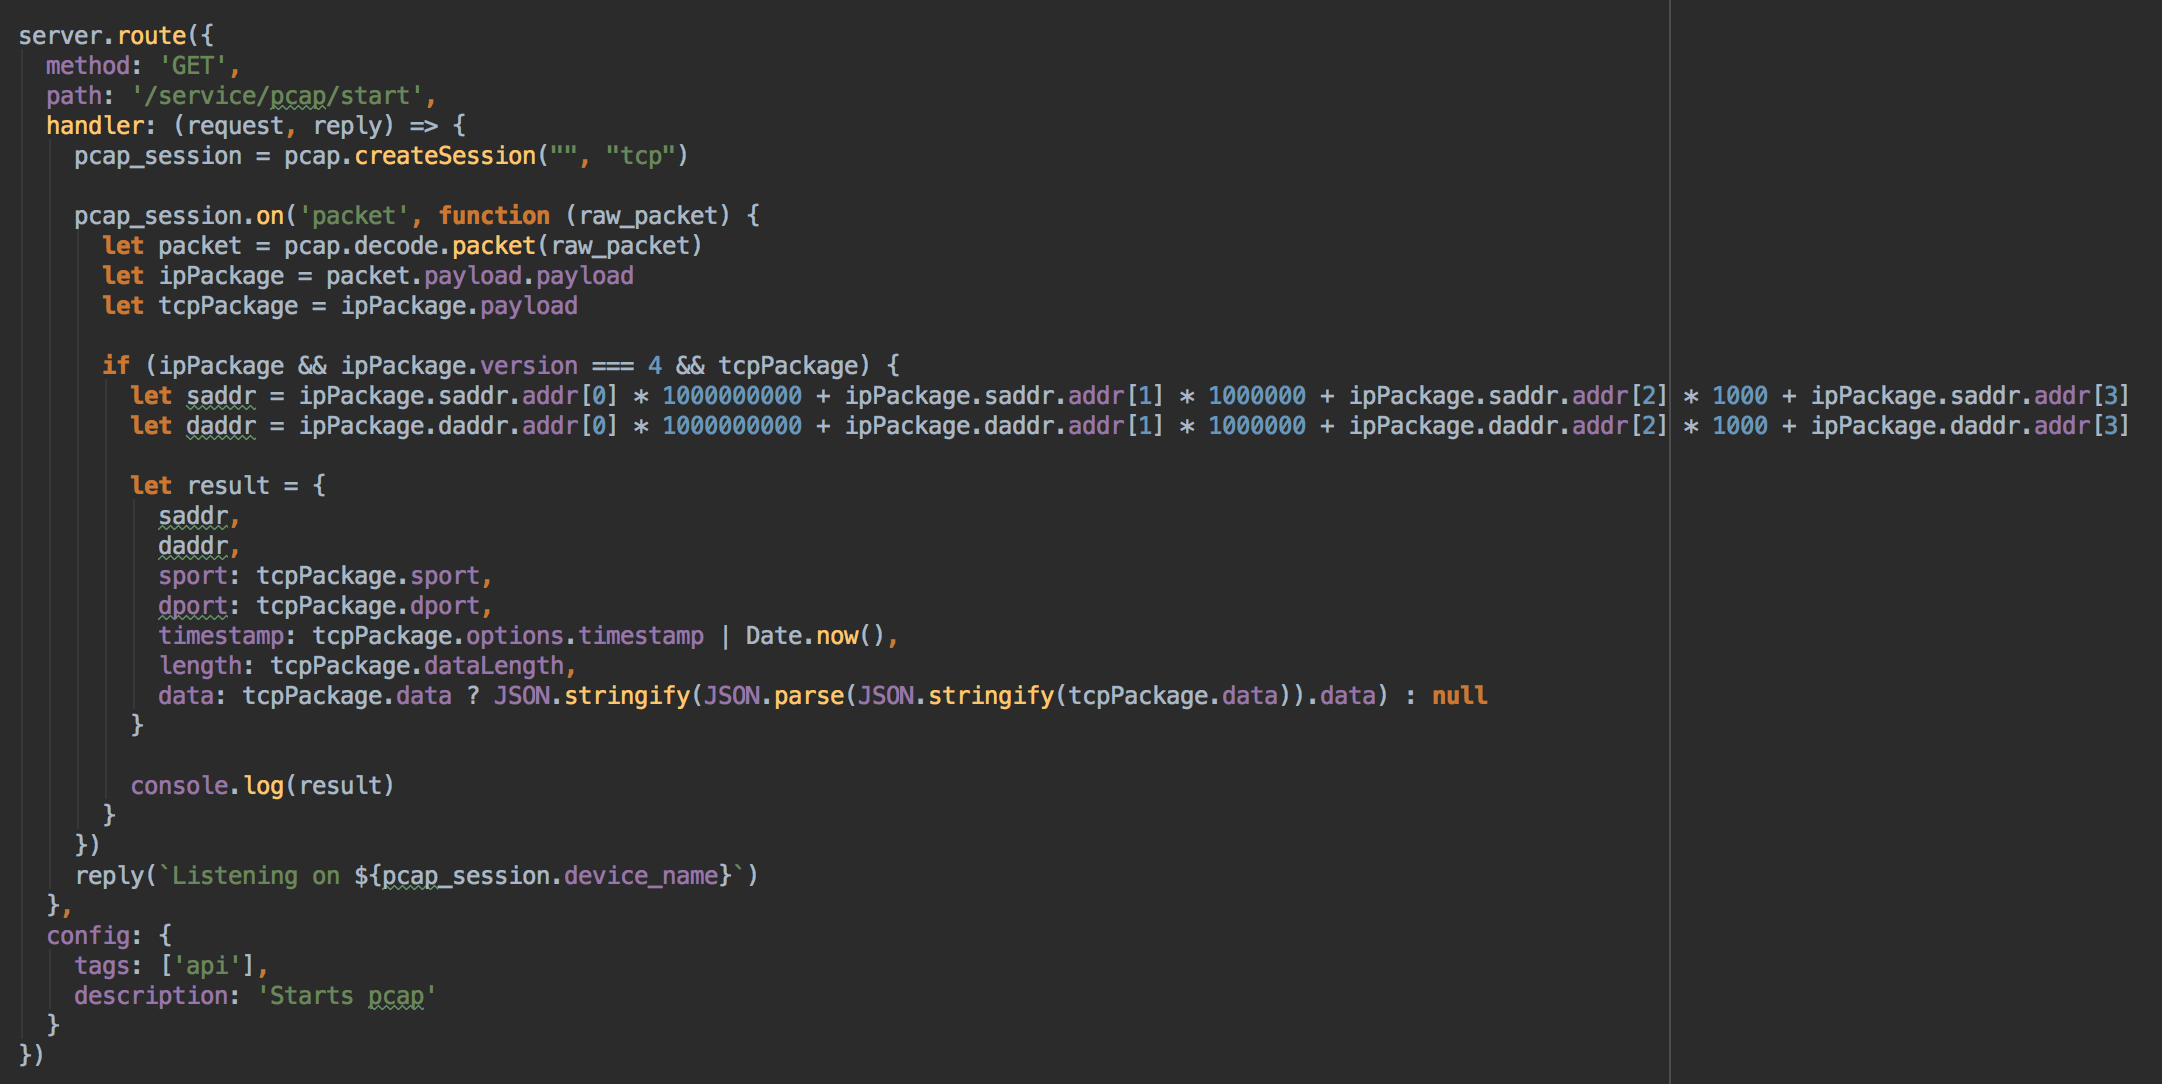
\includegraphics[width=1.0\textwidth]{resources/solution2-1.png}}
	\caption{Network Sniffer Loop}
		\label{loop}
\end{figure}
As there is no general structure more a per query based implementation we will look at each query individually. Every operation focuses on what is being asked for. Splitted in two factors, what wants the user as an output and what do he needs to put into the query. The key is generally a combination of the query name and the parameters put in. We also convert ips to integers as planned to use range functions provided by redis.

\section{Query 1}
The input is a simple timestamp. The user wants all connections around that timeframe. So we created a sorted list called “timestamp” with a timestamp key (\ref{query1}). The value is a combination of source and destination address with the used ports. The output uses a redis query “between” to achieve the wanted one second timeframe (\ref{query11})..

  \begin{figure}[H]
	\centerline{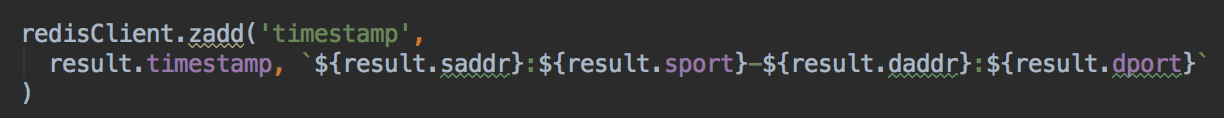
\includegraphics[width=1.0\textwidth]{resources/solution2-2.png}}
	\caption{Fill redis with timestamps}
	\label{query1}
\end{figure}

  \begin{figure}[H]
	\centerline{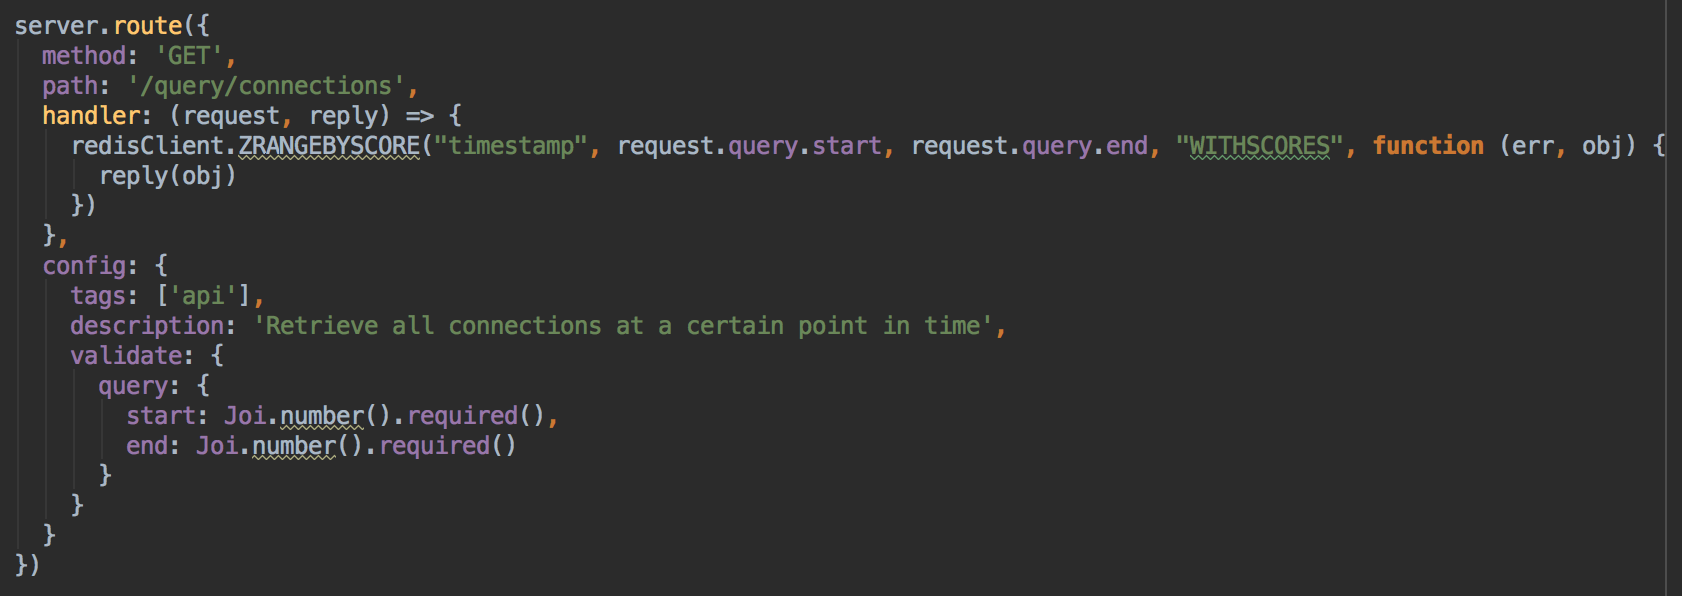
\includegraphics[width=1.0\textwidth]{resources/solution2-3.png}}
	\caption{Query specific timeframes}
	\label{query11}
\end{figure}

\section{Query 2}
The inputs are two different ips. The user wants the overall data volume per minute between those ips. We created a hash storing three values. The start time which is only set once and never changes. A stop time which is set whenever a new fitting connection was found. And a dataSum property which increments with every further fitting connection. Some post processing has to be done here. We need to check both connection directions and a conversion to data volume per minute.

  \begin{figure}[H]
	\centerline{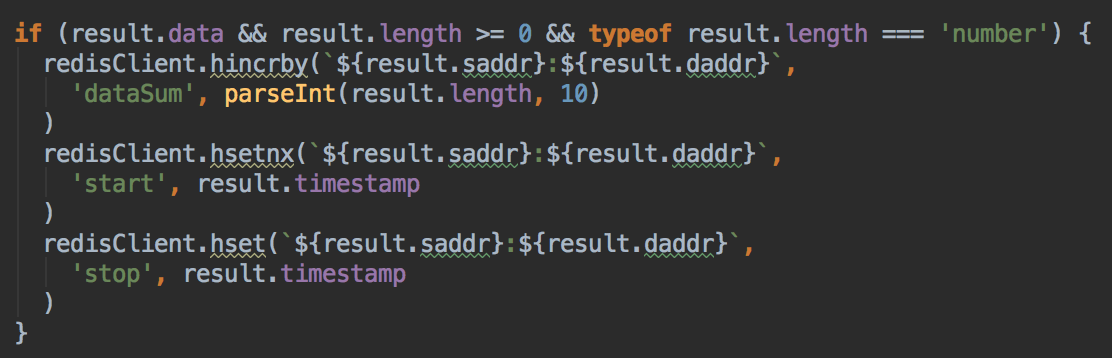
\includegraphics[width=1.0\textwidth]{resources/solution2-4.png}}
	\caption{Fill redis with meta data concerning the data}
	\label{query2}
\end{figure}

\begin{figure}[H]
	\centerline{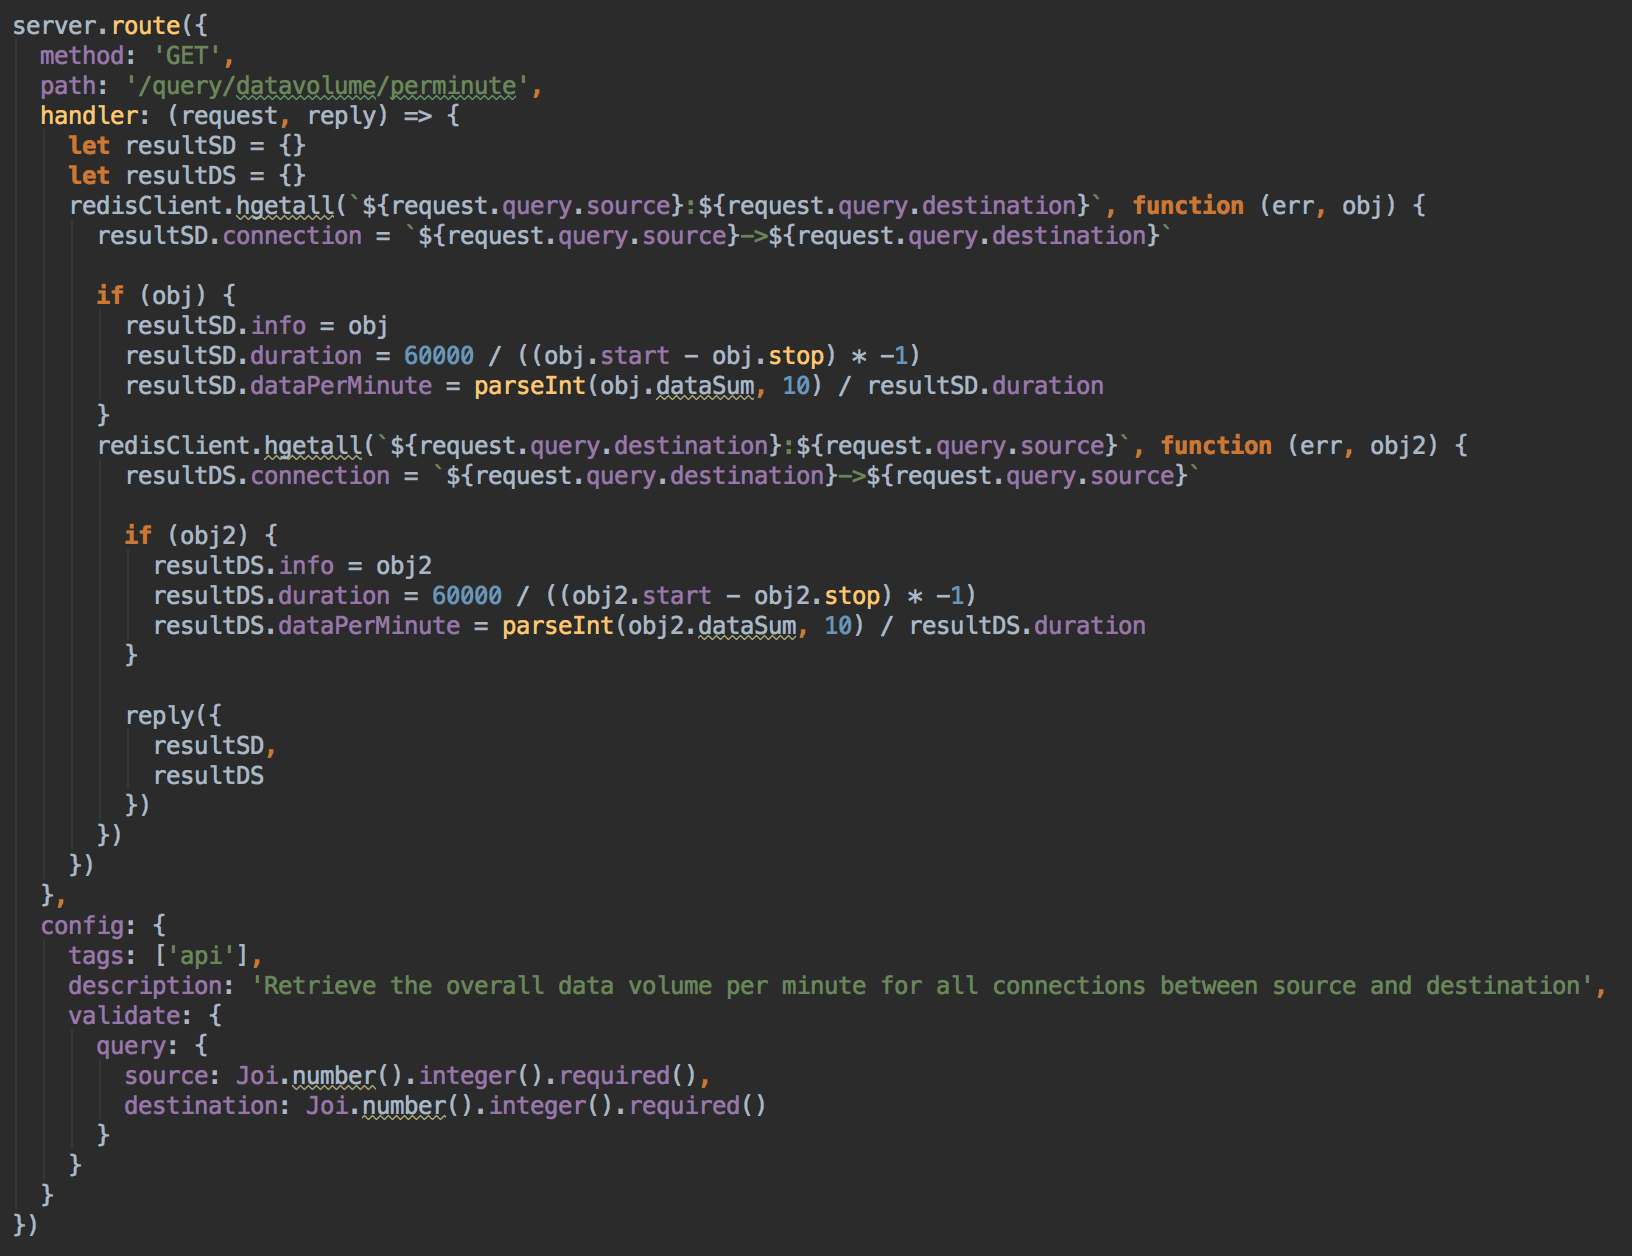
\includegraphics[width=1.0\textwidth]{resources/solution2-5.png}}
	\caption{Query data volume over several packets}
	\label{query22}
\end{figure}

\section{Query 3}
The inputs are an ip address as a destination and a port. In this case HTTP port which is 80 but we wanted some room. The user wants all hosts that this combination had connections to. We created several lists called “hosts” followed by the input combination. A valid list name could be “hosts:201.2.2.1:80”. The values are source addresses. Addresses that had connections to this specific connection. The output is then a generated query via the input followed by all the values within this specific list.

  \begin{figure}[H]
	\centerline{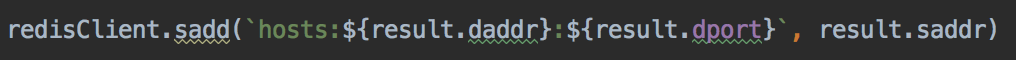
\includegraphics[width=1.0\textwidth]{resources/solution2-6.png}}
	\caption{Fill redis with hosts}
	\label{query3}
\end{figure}

\begin{figure}[H]
	\centerline{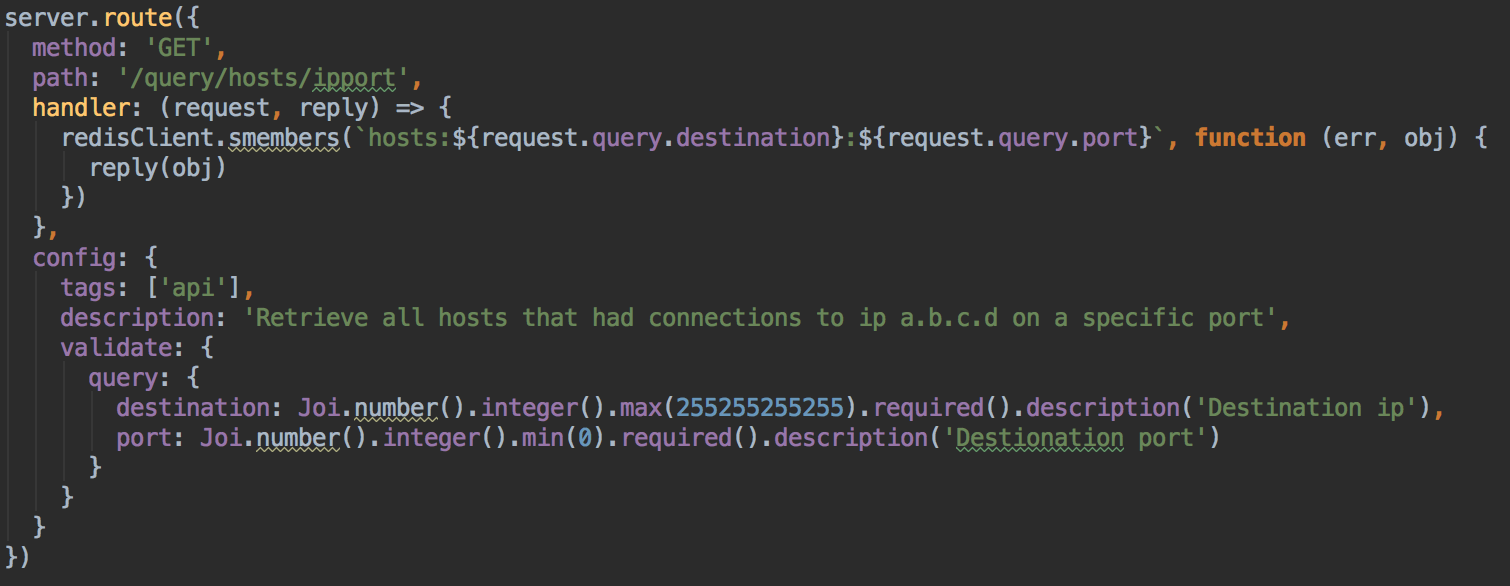
\includegraphics[width=1.0\textwidth]{resources/solution2-7.png}}
	\caption{Query specific hosts}
	\label{query33}
\end{figure}

\section{Query 4}
The input is a start port and an end port. We wanted all connections that had incoming connections to well-known ports. Which means ports that are lower or equal to 1024. This was ideal for redis between. So we used a sorted list called “ports”. The key was the port and the value the destination address. The query simple asked for every key that was lower or equal to 1024.

  \begin{figure}[H]
	\centerline{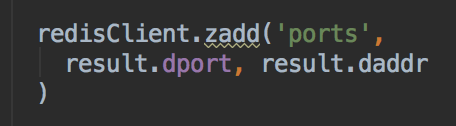
\includegraphics[width=0.5\textwidth]{resources/solution2-8.png}}
	\caption{Fill redis with ports}
	\label{query4}
\end{figure}

\begin{figure}[H]
	\centerline{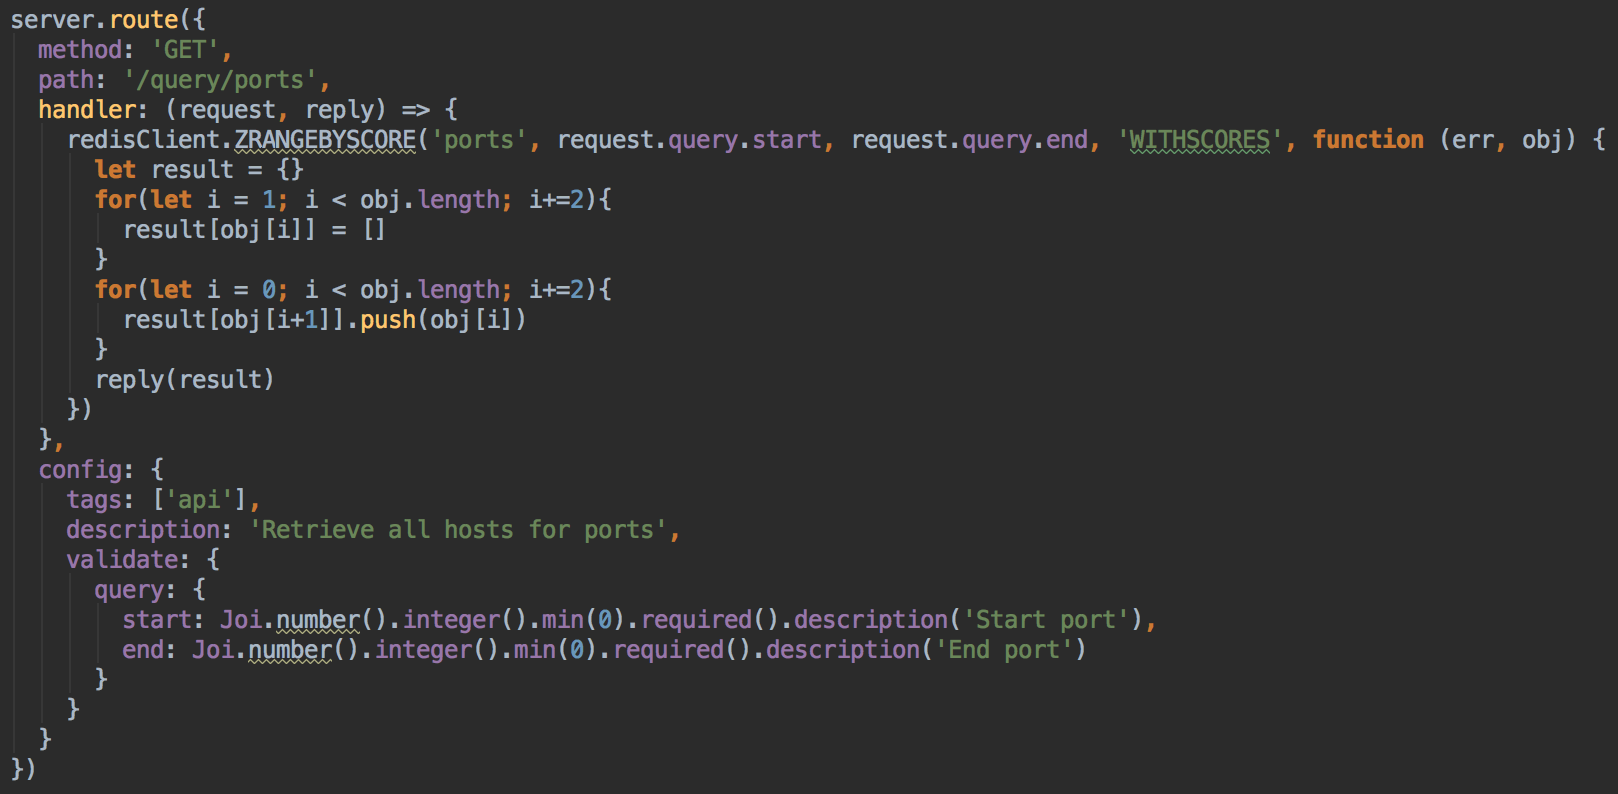
\includegraphics[width=0.8\textwidth]{resources/solution2-9.png}}
	\caption{Query specific port ranges}
	\label{query44}
\end{figure}

\section{Query 5}
The user input is a decimal sequence. Due to technical limitation we can’t scan for a hex sequence. We created list called “data” holding all the packet data. We needed some pre processing in order to make this value searchable. The output starts a redis method called sscan which scans a list with a given regex and returns all packets that meet this criteria.

  \begin{figure}[H]
	\centerline{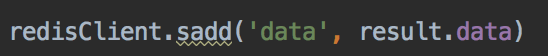
\includegraphics[width=1.0\textwidth]{resources/solution2-10.png}}
	\caption{Fill redis with data blobs}
	\label{query5}
\end{figure}

\begin{figure}[H]
	\centerline{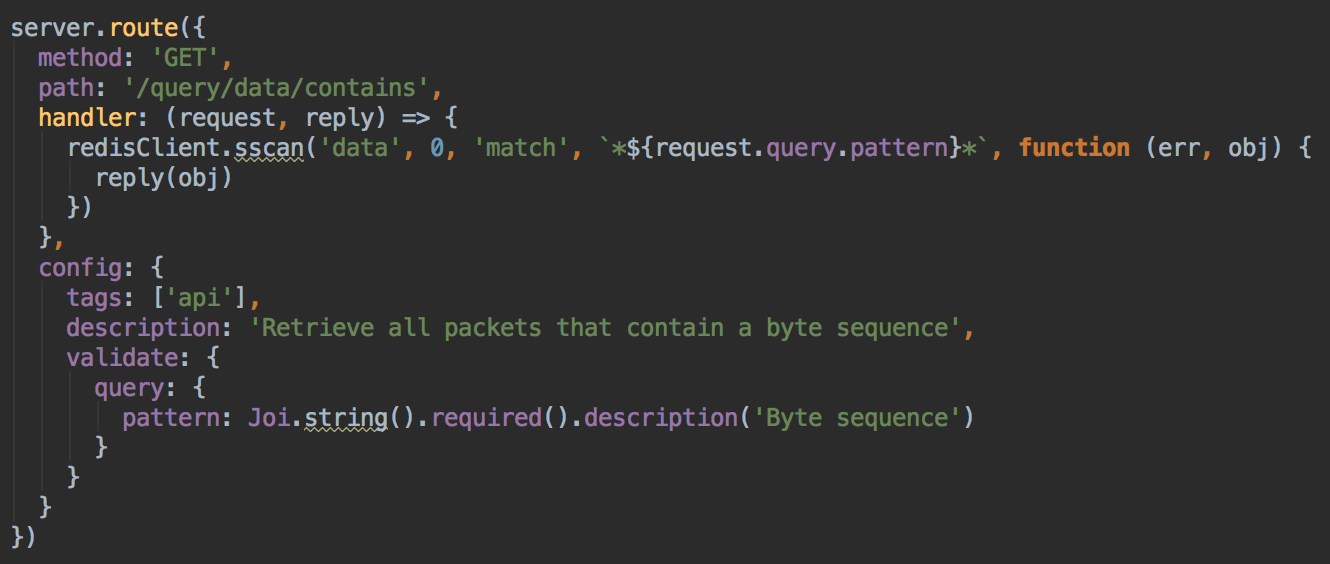
\includegraphics[width=1.0\textwidth]{resources/solution2-11.png}}
	\caption{Query specific data fragments}
	\label{query55}
\end{figure}

\section{Query 6}
The input is nothing. We wanted all hosts that had connections to outside hosts. We created a sorted list called “connections” where the key is the destination address and the value is the source address. The output queries via zrangebyscore every key that fits between a numeric range representing public ips.

  \begin{figure}[H]
	\centerline{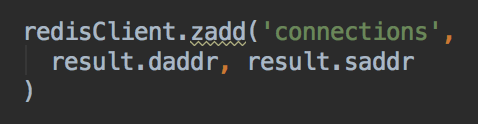
\includegraphics[width=1.0\textwidth]{resources/solution2-12.png}}
	\caption{Fill redis with connections}
	\label{query6}
\end{figure}

\begin{figure}[H]
	\centerline{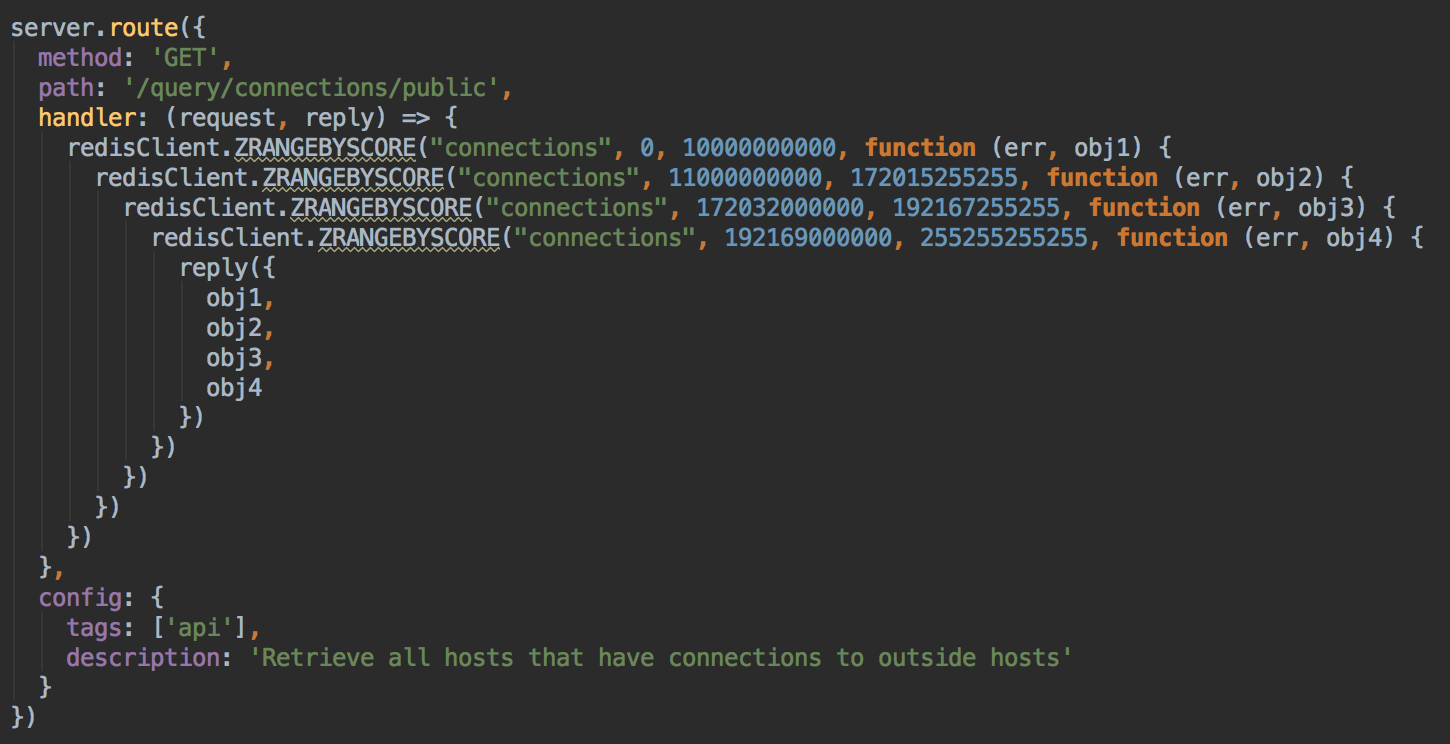
\includegraphics[width=1.0\textwidth]{resources/solution2-13.png}}
	\caption{Query all outside connections}
	\label{query66}
\end{figure}

As you can see this approach is very tight binded to its queries. Some allow a little more freedom and some none. If the application should grow the sniff loop needs to grow as well. Old data may not be suitable for further new queries.

\chapter{Store all with partial redundancy and without post-processing}
This solution was realized with the underlying programming language Python. Redis-py servers as the essential client. The solution does not dissociate from the original plan very much. It is based on the usage of Hashes to store each ethernet packet. At first all attributes on all layers of an ethernet packet are extracted by using a pcap reader in this case pyshark. These extracted values are assigned to variables afterwards. As planned to check whether an IP is private or not is pre-processed likewise if a port is a http or well-known. But instead of using an boolean type here, a simple integer value 1 or 0 is selected. This is for the later explained indexes. Then a hash object will be generated. This hash object stores the following attributes:

\begin{itemize}
	\item source address
	\item source port
	\item destination address
	\item destination port
	\item packet length
	\item timestamp
\end{itemize}

The amount of stored attributes is less than initially intended to store. Like stated in the original plan each hash gets an index and a name operating as the key identifying a single hash. As name the simple string “eth” is chosen. The index is a simple numerical index incremental rising and append to the name of the hash. So each hash object is unique and can be addressed correctly. Diverging from the plan no hash field gets an own index. It is not necessary. Each hash field consists of a name as a key to access this field and the assigned value. An example is shown in the picture:

\begin{figure}[H]
	\centerline{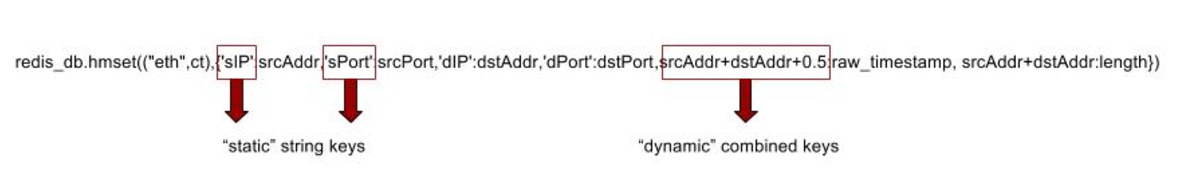
\includegraphics[width=1.0\textwidth]{resources/solution3-1.png}}
\end{figure}

As seen the hash object is created like it was primarily planned. There are two different field keys defined. The “statical” is a simple string which has always the same name. The “dynamically” ones are combined out of two variables holding the extracted source and destination address. The name as the key is the sum of these addresses as integers. So each hash object has a different field name here. Why it is done this way is explained later in the document. 
Having all essential attributes stored, it continues with preparing another Redis data type for the queries derived from the scenario. In order to perform these special queries or any query at all sorted sets are needed. This also a new aspect which was not indicated in the original plan. These sorted sets are the main lists which retrieve the stored hash objects as the result of a query. So sorted sets can hold the same values which leads to partial redundancy. An example of such a sorted set is shown in the following:\\

\begin{center}
zadd('DPwK', dstPort_wellKnown,(redis_db.hmget(('eth',ct),'sIP','sPort')))\\
\end{center}

A sorted set gets a unique name “DPwK” as its key. The second parameter is the previously pre-processed value functioning as the index for the queries. The third one is a reference to the hash objects and particular fields of this hash object depending on the query. Using this reference overwrites any already existing value in the sorted set which leads to natural filtering duplicates - duplicates are not given and each value occurs only once. A reference nested into a sorted list is what was described as a complex data structure back in the basics and makes Redis very flexible when it comes to various kinds of queries. The example seen above points out that the sorted set retrieve all hash objects and its hash fields generated where the corresponding ethernet packet has a well-known destination port. There can be numerous sorted sets to cover any query. The general approach is displayed below:

\begin{figure}[H]
	\centerline{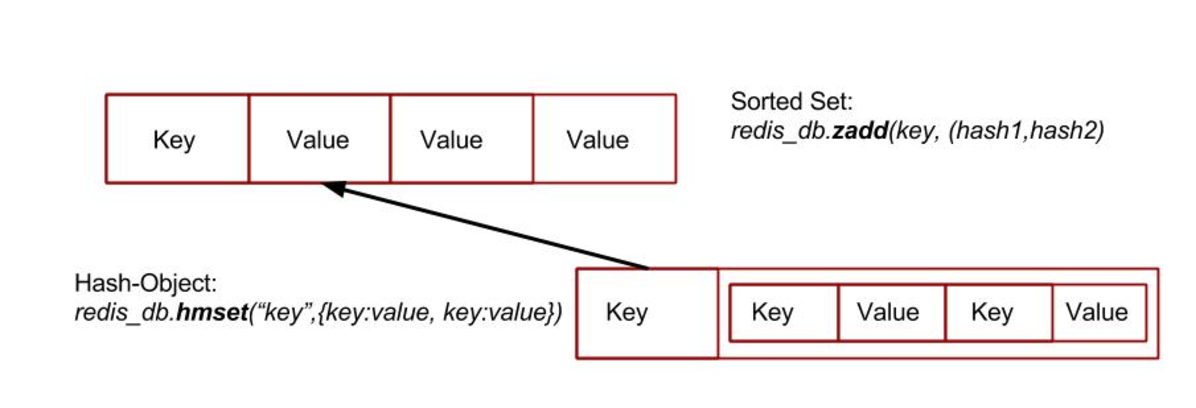
\includegraphics[width=1.0\textwidth]{resources/solution3-2.png}}
\end{figure}

Next follows the queries. As mentioned Redis provides complex data structures which can be accessed by simple commands. A further advantage of Redis. Basing on the example a query to retrieve all hosts that have a connection to a well-known port could be read like:\\

\begin{center}
zrangebyscore('DPwK',1,1)\\
\end{center}

The command “zrangebyscore” enables to retrieve a bunch of stored hash objects with the same score. Therefore Redis first looks which key to access. This is defined in the first parameter of the command. So Redis searches for the sorted set with the name “DPwK” as its key. The second and third parameter define the limitation of the score range. Both are 1 meaning that all sorted sets with a score of 1 should return their values. “zrangebyscore” needs float or integer values to operate. That’s why integers instead of booleans were selected while pre-processing if a port is well-known. The found sorted sets return their values. These values are references to hash objects generated when the pre-processed variable \begin{comment}
	"dstPort{\_}wellKnown"
\end{comment} was 1. 

\begin{figure}[H]
	\centerline{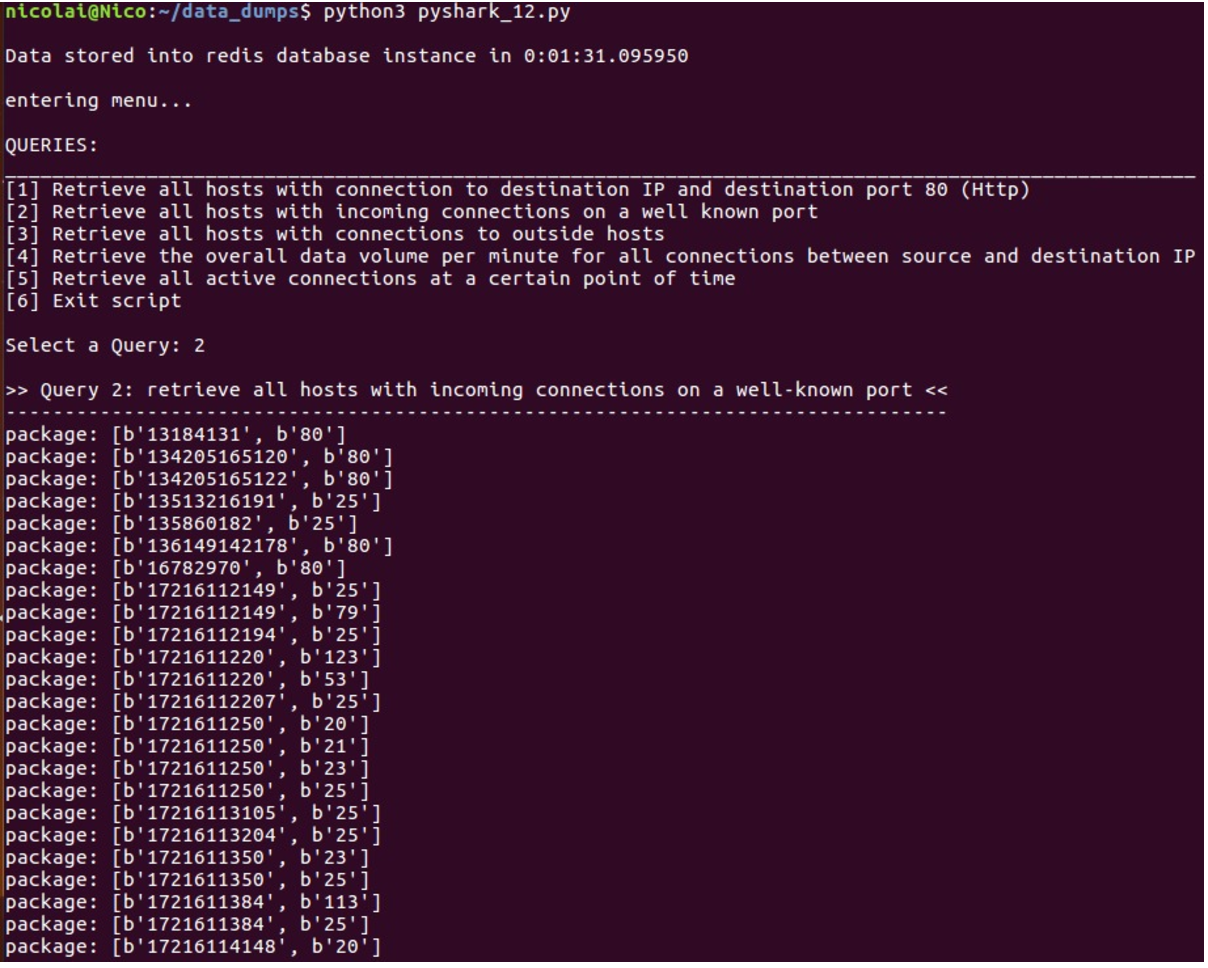
\includegraphics[width=1.0\textwidth]{resources/solution3-3.png}}
\end{figure}

The screenshots shows the result of the query for all well-known ports. Each package exists only once due to filtering duplicates and consists of the destination address and the destination port belonging to the hash object which fulfills the querying criteria.\\
Every query in this solution works the same. It shows what Redis is capable of in mind that Redis provides many options and commands. The only post-processing necessary is facing the query to retrieve the overall data volume per minute between two IPs. All in all this solution is rather simple and does not exploit the full capability of Redis. Nevertheless it is sufficient.

\chapter{Conclusion}
Every of our solutions works fine and are actually build on one another. Through the working process we came to the final conclusion that we would recommend rather the last solution. This one allows to store everything we want and retrieve any data depending on the desired query. It aims for the native language of Redis and can therefore be implemented with any technology around. Its complexity is low. You only need to read the Redis documentation for understanding what we have done. All in all it mirrors our learning progress. This progress does not end with this final solution knowing there are many possibilities provided by Redis (e.g. Lua Script) we did not use. 


% bibliography
% Wichtig: Das Literaturverzeichnis steht ganz am Ende der Arbeit, also nach
% einem möglichen Anhang.
\renewcommand{\btxfnamespaceshort}{\,}
\bibliographystyle{bababbrv_unsrt}

\end{document}
